%----------------------------------------------------------------------------------------
%	CONSTANTS
%----------------------------------------------------------------------------------------

\newcommand{\hmwkTitle}{Report\ \#2}					% Assignment title
\newcommand{\hmwkClass}{Communication Networks}			% Course name
\newcommand{\hmwkClassTime}{}							% Workshop time
\newcommand{\hmwkClassInstructor}{}						% Tutor name
\newcommand{\hmwkAuthorName}{Ang LEE}					% Student name

\newcommand{\hmwkGraphicsPath}{img/}					% Graphics path

%----------------------------------------------------------------------------------------
%	TEMPLATE
%----------------------------------------------------------------------------------------

\documentclass{article}

\usepackage{fancyhdr}	% Required for custom headers
\usepackage{lastpage}	% Required to determine the last page for the footer
\usepackage{extramarks} % Required for headers and footers
\usepackage{graphicx}	% Required to insert images
\graphicspath{\hmwkGraphicsPath}
\usepackage{lipsum} 	% Used for inserting dummy 'Lorem ipsum' text into the template

\usepackage{float}
\usepackage{epstopdf}	% Required to insert .eps images
\usepackage{amssymb}
\usepackage{amsmath}
\usepackage[hidelinks]{hyperref}

% Python syntax highlighting
\usepackage{color}		% Required to define colors
\definecolor{commentColor}{RGB}{153,153,153}
\definecolor{stringColor}{RGB}{37,170,33}
\usepackage{listings}
\lstset{
	language=Python,
	basicstyle=\footnotesize\ttfamily,
	keywordstyle=\color{blue},
	stringstyle=\color{stringColor},
	commentstyle=\usefont{T1}{pcr}{m}{n}\color{commentColor},
	breaklines=true,
	showstringspaces=false
}

% Margins
\topmargin=-0.45in
\evensidemargin=0in
\oddsidemargin=0in
\textwidth=6.5in
\textheight=9.0in
\headsep=0.25in

\linespread{1.1}		% Line spacing

% Set up the header and footer
\pagestyle{fancy}
\lhead{\hmwkTitle} % Header Left 
\chead{\hmwkAuthorName} % Header Center
\rhead{\hmwkClass} % Header Right
\lfoot{\url{https://github.com/leeang/Communication-Networks}} % Footer Left
\cfoot{} % Footer Center
\rfoot{Page\ \thepage\ of\ \pageref{LastPage}} % Footer Right
\renewcommand\headrulewidth{0.4pt} % Size of the header rule
\renewcommand\footrulewidth{0.4pt} % Size of the footer rule

\setlength\parindent{0pt} % Removes all indentation from paragraphs

%----------------------------------------------------------------------------------------
%	Problem and Section
%----------------------------------------------------------------------------------------

\newenvironment{homeworkProblem}[1]{
	\section*{#1}
	}{
}
\newenvironment{homeworkSection}[1]{
	\subsection*{#1}
	}{
}
\newcommand{\problemAnswer}[1]{
	\noindent\framebox[\columnwidth][c]{
		\begin{minipage}{0.98\columnwidth}
			#1
		\end{minipage}
	}
}

%----------------------------------------------------------------------------------------
%	Document
%----------------------------------------------------------------------------------------

\begin{document}

\newpage

%----------------------------------------------------------------------------------------
%	Section 1
%----------------------------------------------------------------------------------------

\begin{homeworkProblem}{Question 1.1}
Briefly discuss socket family and type within the context of the \texttt{socket()} function. What are the differences between the \texttt{SOCK\_STREAM} and \texttt{SOCK\_DGRAM} socket types? In which context would you use one over the other?\\

\problemAnswer{
\vspace{5pt}
\texttt{AF\_UNIX}, \texttt{AF\_INET} and \texttt{AF\_INET6} represent the address (and protocol) families, used for the first argument to \texttt{socket()}.\\

\texttt{SOCK\_STREAM}, \texttt{SOCK\_DGRAM}, \texttt{SOCK\_RAW}, \texttt{SOCK\_RDM} and \texttt{SOCK\_SEQPACKET} represent the socket types, used for the second argument to \texttt{socket()}. (Only \texttt{SOCK\_STREAM} and \texttt{SOCK\_DGRAM} appear to be generally useful.)\\

\texttt{SOCK\_STREAM} provides sequenced, reliable, two-way, connection-based byte streams. An out-of-band data transmission
mechanism may be supported.\\
\texttt{SOCK\_DGRAM} supports datagrams (connectionless, unreliable messages of a fixed maximum length).\\

For small messages with known upper bound on message length, e.g. UDP broadcasts sends are always enabled on a datagram socket, \texttt{SOCK\_DGRAM} is recommended.\\
For arbitrary long message payloads such as file tranfer, \texttt{SOCK\_STREAM} would be better.
}

Reference:\\
\url{https://docs.python.org/2/library/socket.html}\\
\url{http://man7.org/linux/man-pages/man2/socket.2.html}
\end{homeworkProblem}


\begin{homeworkProblem}{Question 1.2}
What is the purpose of the \texttt{socket.bind()} function in the Python socket module? What is the format of the address parameter in the \texttt{AF\_INET} case? Would you use this function when implementing a server, a client or both? Justify your answer.\\

\problemAnswer{
\vspace{5pt}
Bind the socket to address.\\

A pair \texttt{(host, port)} is used for the \texttt{AF\_INET} address family, where host is a string representing either a hostname in Internet domain notation like `\texttt{www.unimelb.edu.au}' or an IPv4 address like `\texttt{8.8.8.8}', and port is an integer.\\

I would not use this function when implementing a client, primarily because if a socket does not call \texttt{bind()}, the operating system will automatically assign an ephemeral port. However, on servers, well-known ports are used by system processes that provide widely used types of network services, e.g. 80 for HTTP, 22 for SSH, 53 for DNS. \texttt{bind()} function is called in order to agree with official assignments of port numbers for specific uses.
}
\end{homeworkProblem}


\begin{homeworkProblem}{Question 1.3}
Which functions of the socket API would you need to implement a simple server using a connectionless mode of communication? Which functions of the socket API would you need to implement a simple server using a connection oriented mode of communication?\\

\problemAnswer{
\vspace{5pt}

\begin{homeworkSection}{Connectionless (UDP)}
Socket type: \texttt{SOCK\_DGRAM}\\
\texttt{socket()}, \texttt{bind()}, \texttt{sendto()}, \texttt{recvfrom()}, \texttt{close()}

\begin{figure}[H]
\centering
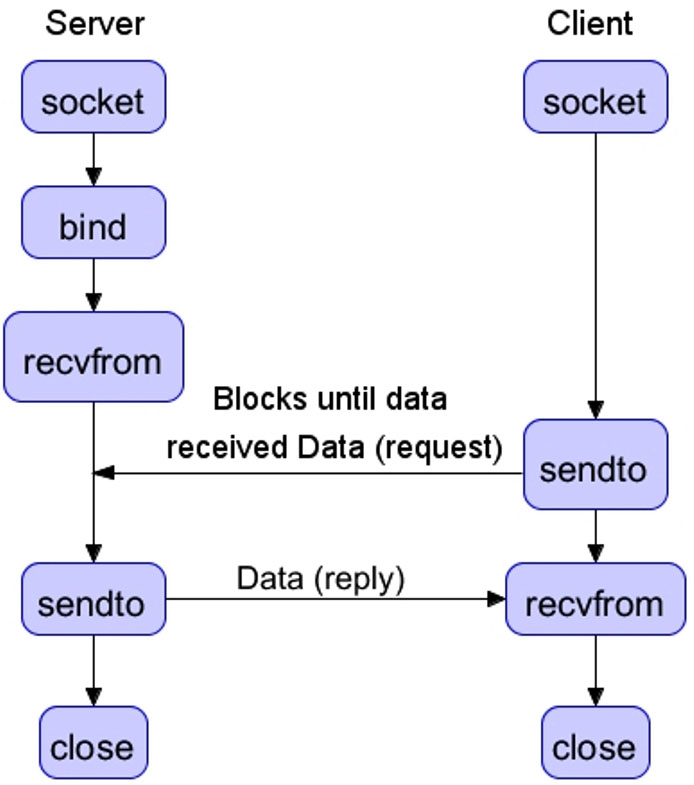
\includegraphics[width=2in]{img/udp_socket}
\caption{APIs for UDP Server/Client}
\end{figure}
\end{homeworkSection}
}

\vspace{10pt}
\problemAnswer{
\vspace{5pt}
\begin{homeworkSection}{Connection-oriented (TCP)}
Socket type: \texttt{SOCK\_STREAM}\\
\texttt{socket()}, \texttt{connect()}, \texttt{bind()}, \texttt{listen()}, \texttt{accept()}, \texttt{send()}, \texttt{recv()}, \texttt{close()}

\begin{figure}[H]
\centering
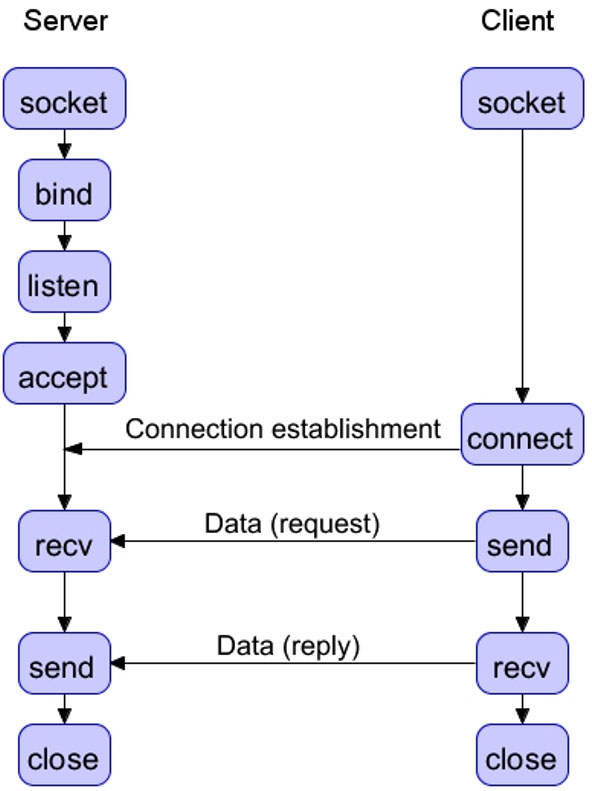
\includegraphics[width=2in]{img/tcp_socket}
\caption{APIs for TCP Server/Client}
\end{figure}
\end{homeworkSection}
}

Reference:\\
\url{https://docs.python.org/2/library/socket.html#socket-objects}\\
\url{http://liuj.fcu.edu.tw/net_pg/socket.html}

\end{homeworkProblem}


\begin{homeworkProblem}{Question 1.4}
Explain the difference between a blocking and non-blocking socket. Which one is used most commonly in practice?\\

\problemAnswer{
\vspace{5pt}
In non-blocking mode, if a \texttt{recv()} call doesn't find any data, or if a \texttt{send()} call can't immediately dispose of the data, a error exception is raised; in blocking mode, the calls block until they can proceed.\\

Blocking mode is used most commonly in practice.
}

Reference:\\
\url{https://docs.python.org/2/library/socket.html#socket.socket.setblocking}
\end{homeworkProblem}

%----------------------------------------------------------------------------------------
%	Section 2
%----------------------------------------------------------------------------------------

\begin{homeworkProblem}{Question 2.1}
Describe the use and purpose of the following functions, and indicate if they will be used to implement a client, a server or both: (a) \texttt{socket.connect()}, (b) \texttt{socket.listen()}, (c) \texttt{socket.accept()}.\\

\problemAnswer{
\vspace{5pt}
\begin{homeworkSection}{(a) \texttt{socket.connect(address)}}
Connect to a remote socket at \texttt{address}.\\

Implemented on a client, because in most cases, a client initiates a connection.
\end{homeworkSection}

\begin{homeworkSection}{(b) \texttt{socket.listen(backlog)}}
Listen for connections made to the socket. The \texttt{backlog} argument specifies the maximum number of queued connections and should be at least 0; the maximum value is system-dependent (usually 5), the minimum value is forced to 0.\\

Implemented on a server, because servers usually wait to be connected.
\end{homeworkSection}

\begin{homeworkSection}{(c) \texttt{socket.accept()}}
Accept a connection. The socket must be bound to an address and listening for connections. The return value is a pair \texttt{(conn, address)} where \texttt{conn} is a new socket object usable to send and receive data on the connection, and \texttt{address} is the address bound to the socket on the other end of the connection.\\

Implemented on a server. After a client initiates a connection, a server will accept it.
\end{homeworkSection}
}

Reference:\\
\url{https://docs.python.org/2/library/socket.html#socket-objects}

\end{homeworkProblem}


\newpage
\begin{homeworkProblem}{Question 2.2}
Why does \texttt{socket.accept()} return a new socket each time? Should you set it to be blocking or non-blocking in your program (assuming a single threaded server)?\\
\end{homeworkProblem}

\problemAnswer{
\vspace{5pt}
\texttt{socket.accept()}\\
Accept a connection. The socket must be bound to an address and listening for connections. The return value is a pair \texttt{(conn, address)} where \texttt{conn} is a new socket object usable to send and receive data on the connection, and \texttt{address} is the address bound to the socket on the other end of the connection.\\

New sockets should be generated because the original one is used to wait for new connection from other users.\\

Blocking mode should be set in the the program. Once a new client is successfully connected, a new socket will be established. If no connections are pending, \texttt{socket.accept()} will block until next connection comes.
}

\clearpage

%----------------------------------------------------------------------------------------
%	Appendix
%----------------------------------------------------------------------------------------

\begin{homeworkProblem}{Appendix}

%--------------------------------------------

\begin{homeworkSection}{Question 1.5 Server}
\lstinputlisting{section1/server.py}
\end{homeworkSection}

%--------------------------------------------

\newpage
\begin{homeworkSection}{Question 1.5 Client}
\lstinputlisting{section1/client.py}
\end{homeworkSection}

%--------------------------------------------

\newpage
\begin{homeworkSection}{Question 2.3 Server}
\lstinputlisting{section2/server.py}
\end{homeworkSection}

%--------------------------------------------

\begin{homeworkSection}{Question 2.3 Client}
\lstinputlisting{section2/client.py}
\end{homeworkSection}

%--------------------------------------------

\end{homeworkProblem}

%----------------------------------------------------------------------------------------

\end{document}
